\title{McDonald Observatory 2.1m Telescope\\
Observers' Guide}
\author{
        Joshua Reding\\
                Department of Physics and Astronomy\\
        University of North Carolina at Chapel Hill\\
        Chapel Hill, North Carolina
}
\date{\today}

\documentclass[12pt]{article}
\usepackage{graphicx}
\usepackage{textcomp}
\usepackage[margin=1.0in]{geometry}
\begin{document}
\maketitle

\section{Introduction}
This provides a comprehensive guide for using the ARGOS instrument and ProEM Camera on the 2.1m Otto Struve Telescope at McDonald Observatory, Fort Davis, Texas. If you are already familiar with the software and instrument, you may skip to sections~\ref{calibrations} and~\ref{end} for helpful checklists to ensure you begin and end the night without incident.

\paragraph{Outline}
The remainder of this guide is organized as follows:\par
\textit{Section~\ref{telescope operation}} - describes how to operate the telescope.\par
\textit{Section~\ref{lightfield}} - describes the \textit{LightField} data acqusition program.\par
\textit{Section~\ref{calibrations}} - instructs on how to prepare your calibration images for photometry.\par
\textit{Section~\ref{acquisition}} - instructs proper data collection.\par
\textit{Section~\ref{end}} - end of night processes.

\section{Telescope Operation}\label{telescope operation}
The 2.1m telescope may be operated using any of three devices: the main control panel inside the dome, the yellow hand paddle inside the dome, or the yellow hand paddle inside the warm room. All three devices have a built-in safety mechanism, which must be held during operation for the telescope to respond; for the control panel, there is a foot pedal on the floor underneath the console, and for the paddles, there is a trigger button on the reverse side of the handle.\par

\begin{figure}[t]
   \centering
   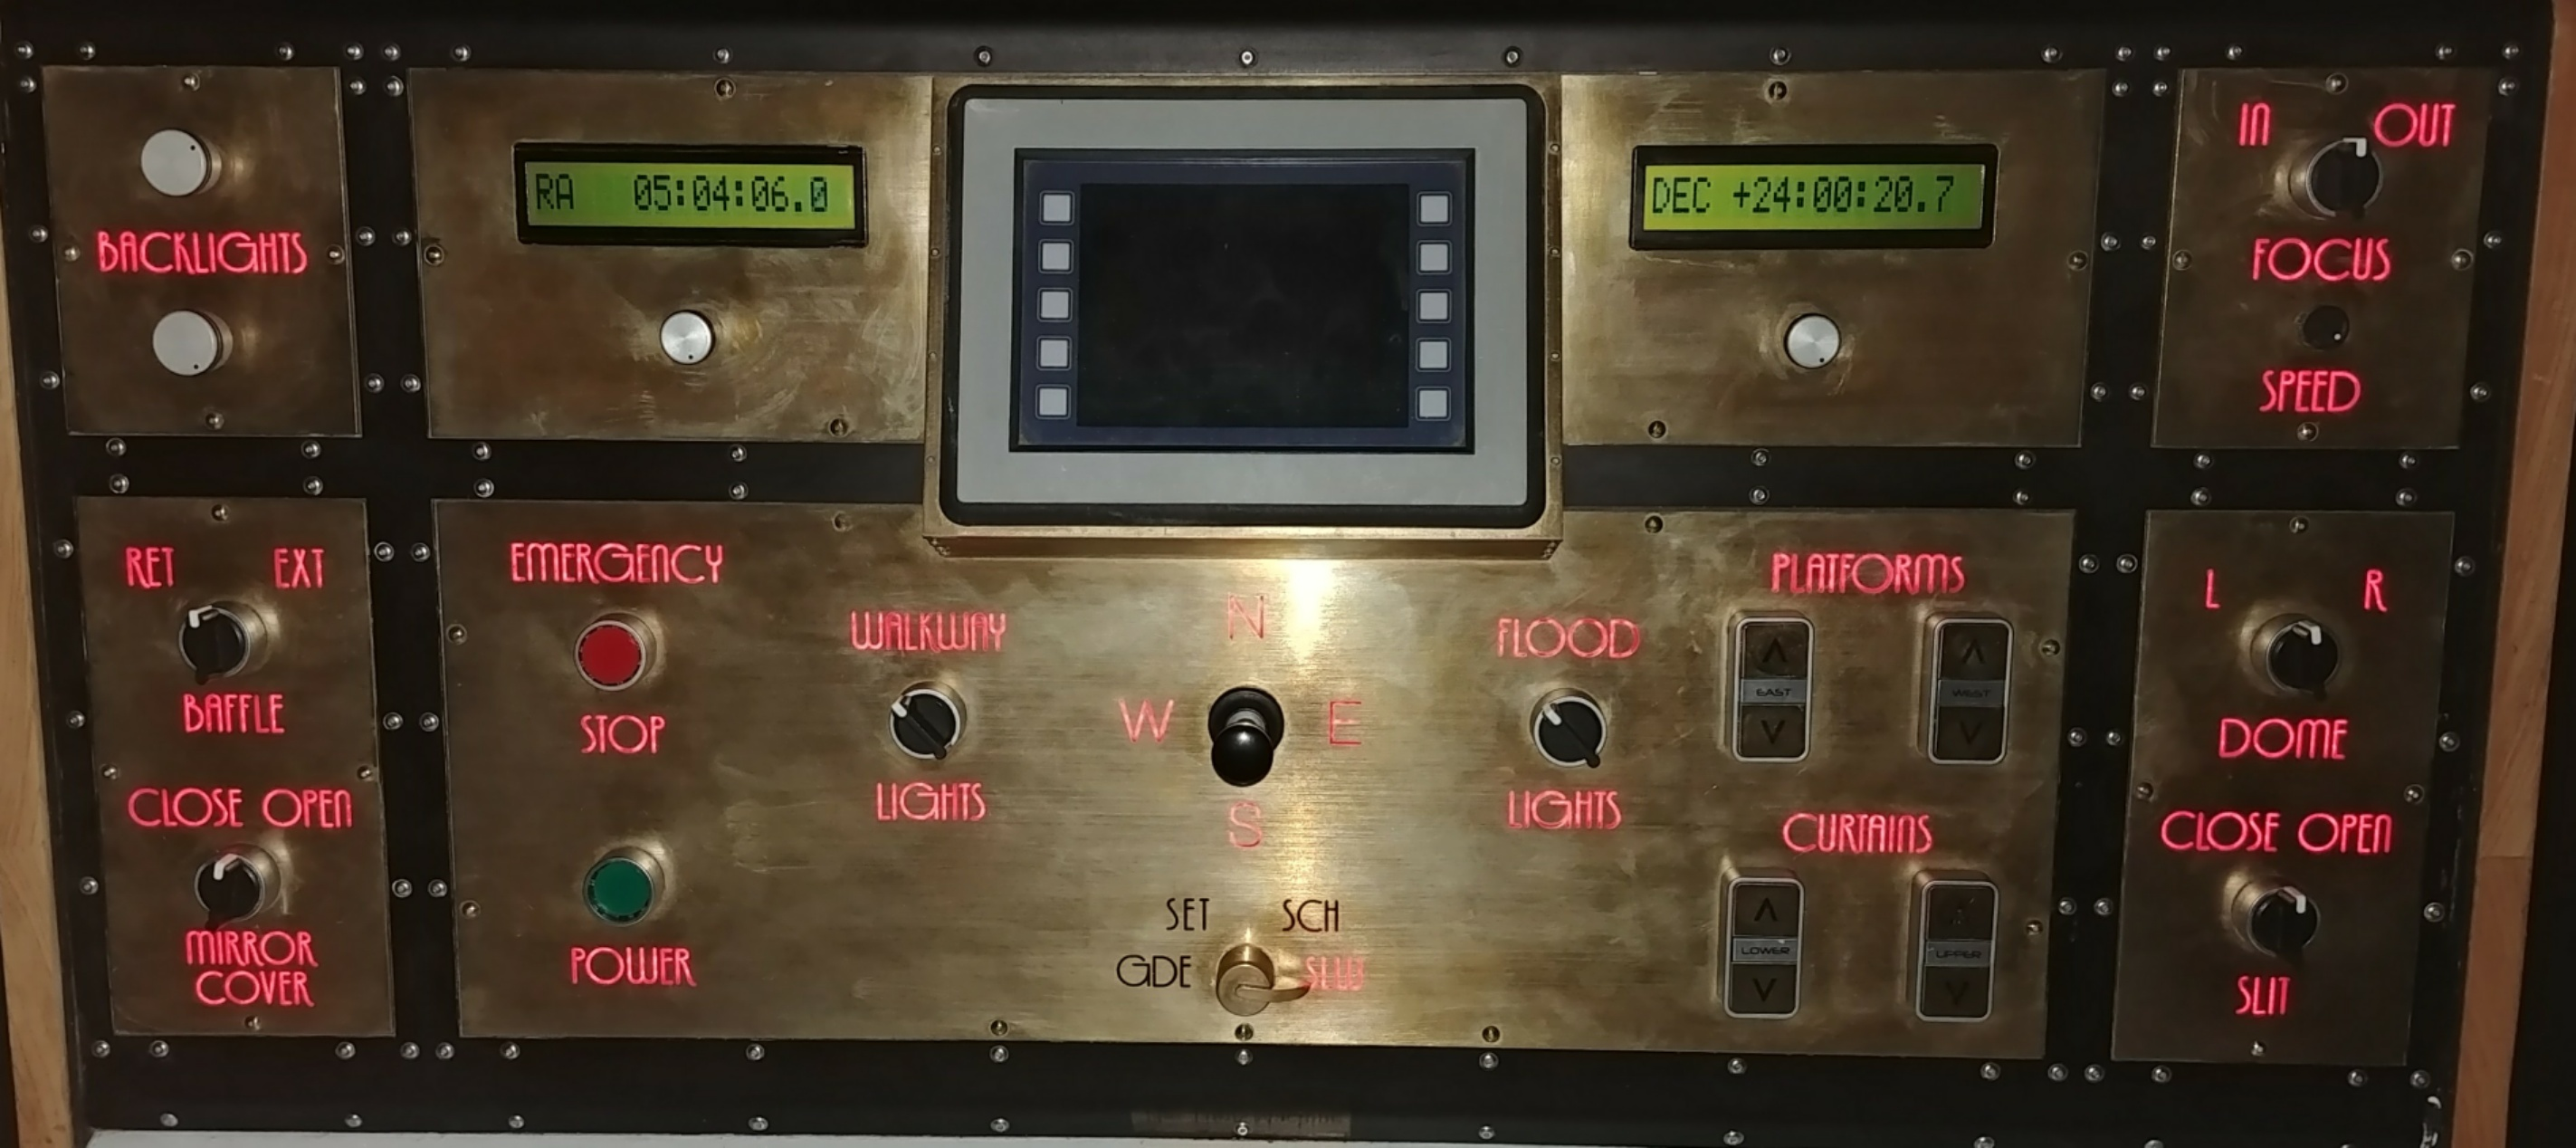
\includegraphics[width=\textwidth]{console.jpg}
   \caption{Main control panel console.\label{fig:console}}
\end{figure}

\begin{figure}[b!]
   \centering
   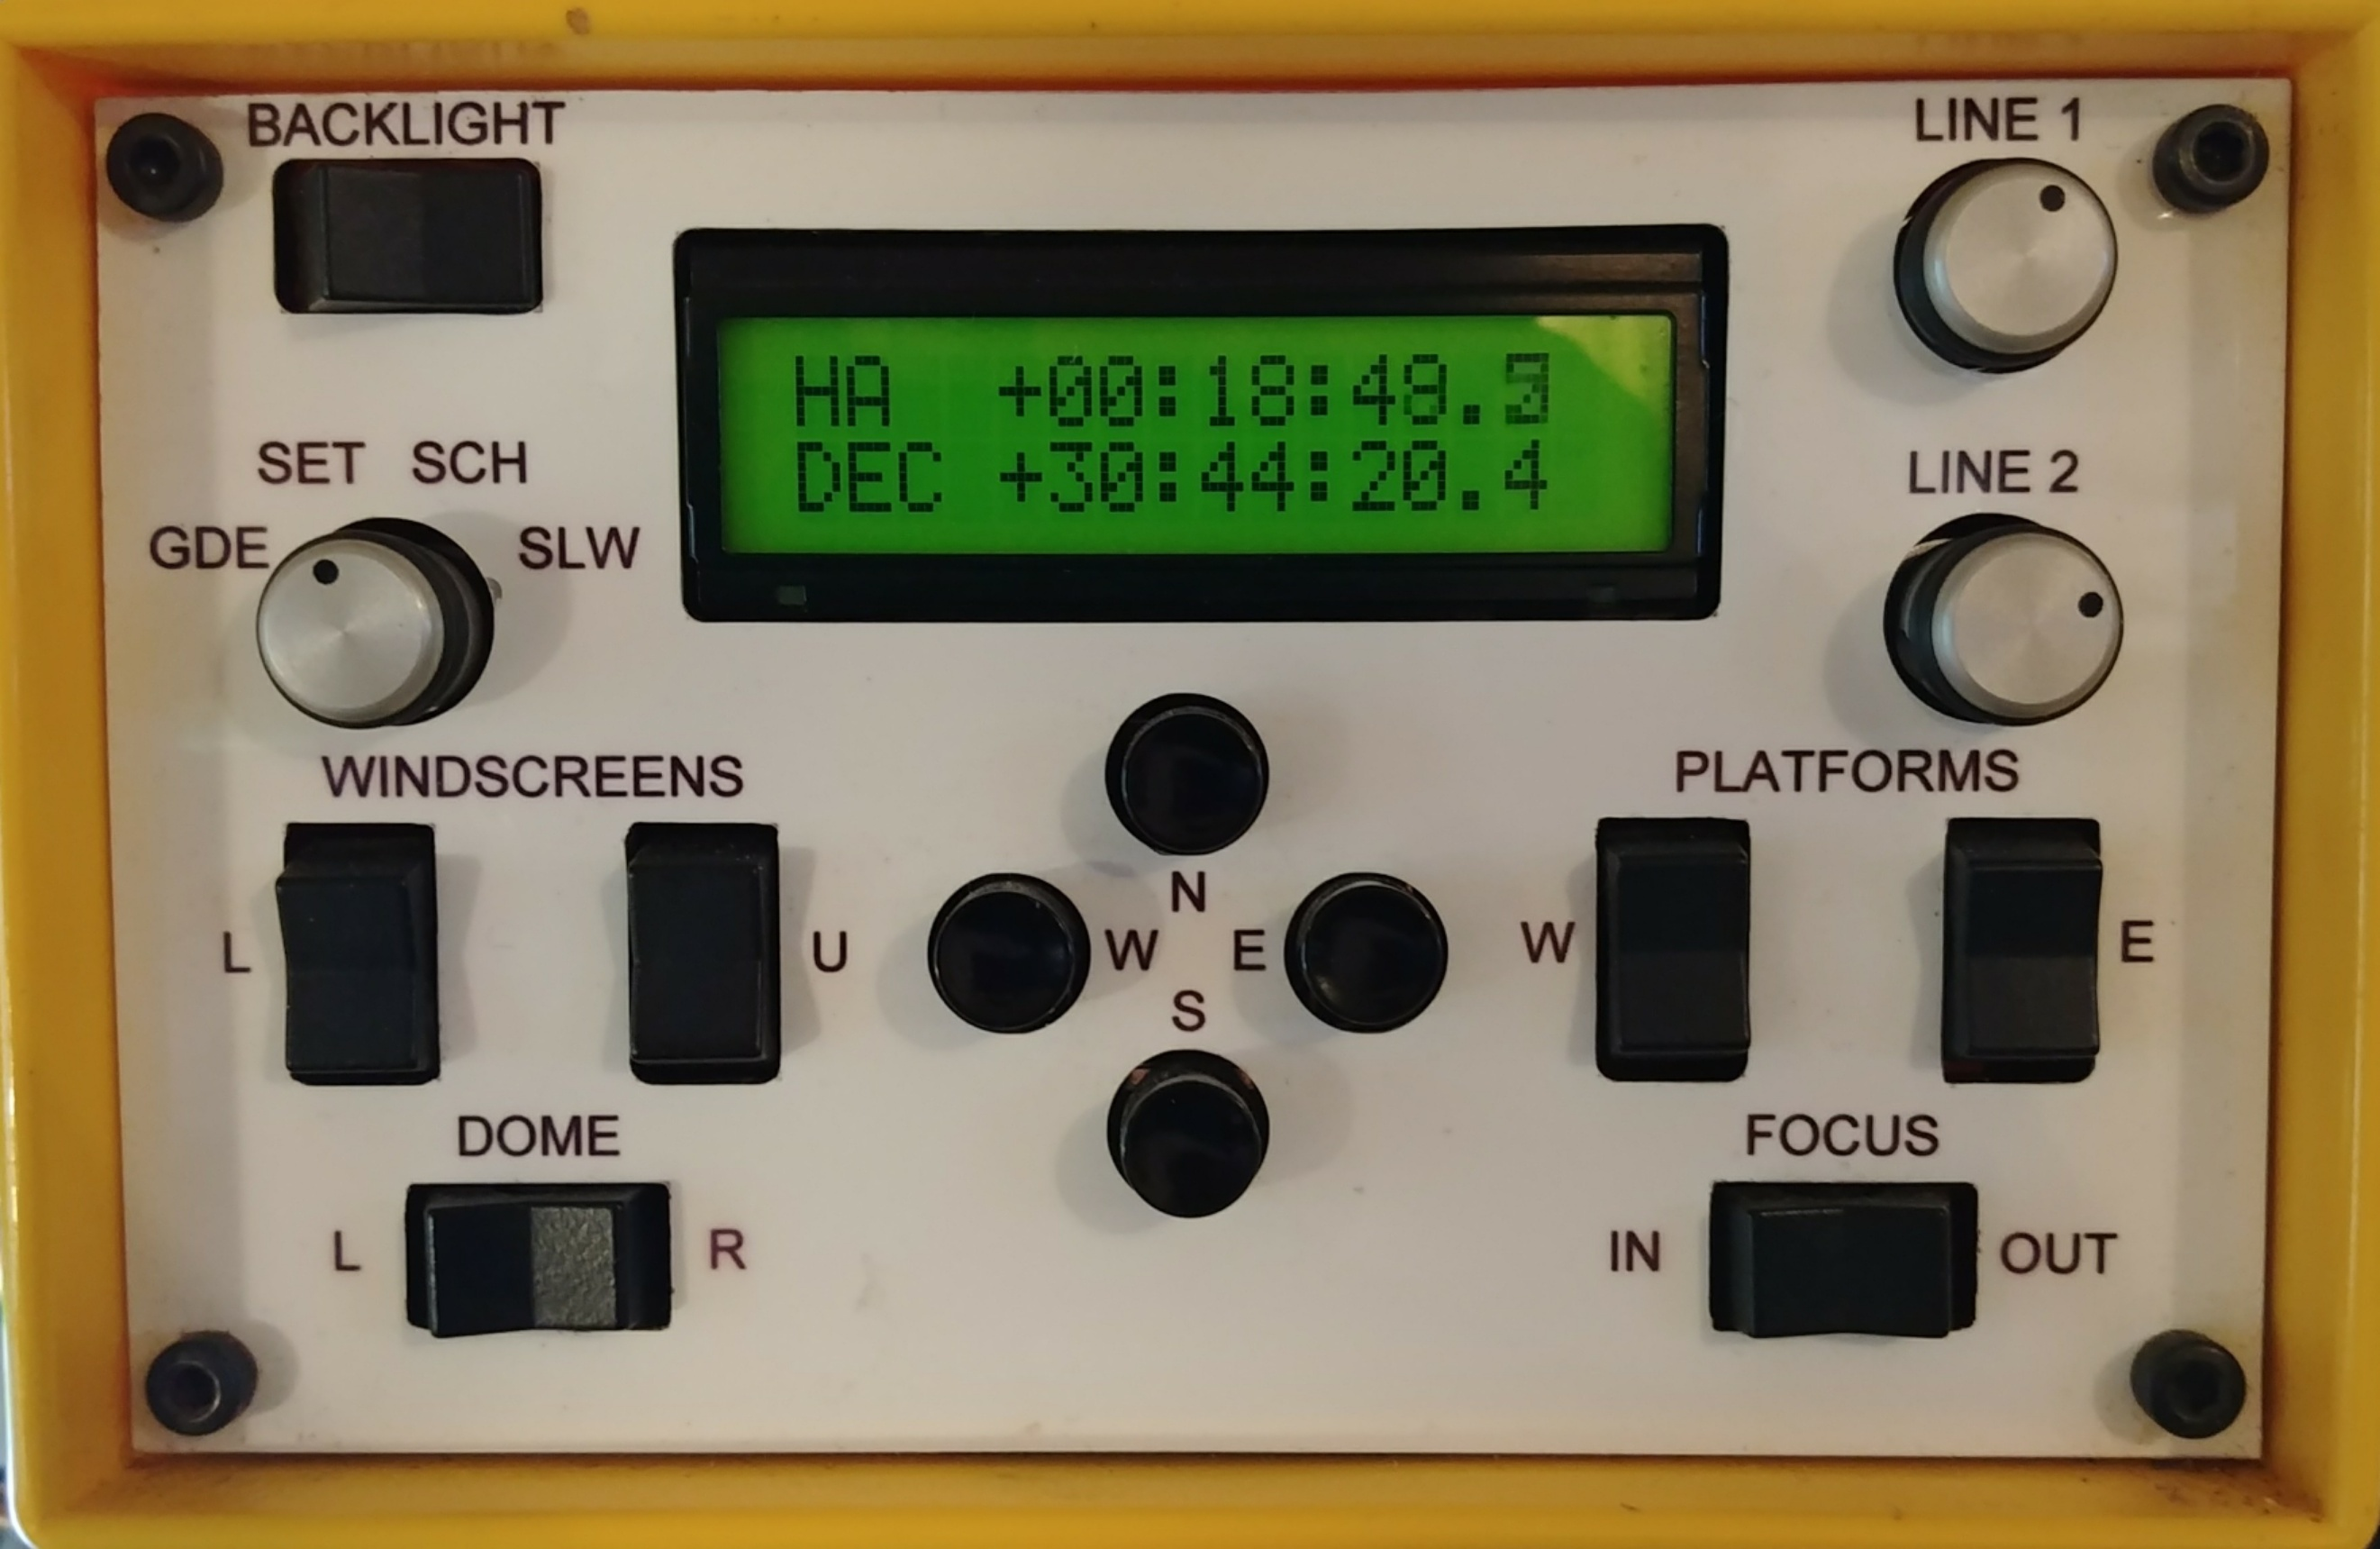
\includegraphics[width=0.5\textwidth]{paddle.jpg}
   \caption{Control paddle interface.\label{fig:paddle}}
\end{figure}

The main control panel is pictured in Figure~\ref{fig:console}. In the top-left, labeled ``BACKLIGHTS,'' the upper knob will illuminate the telescope information screens, while the lower knob illuminates the instruction panel text. Below that are the baffle and mirror cover controls. To the left and right in the upper-central panel are the telescope information screens, which can be adjusted to show values of UT, LST, HA, DEC, RA, and FOC by turning the knobs below the displays. In the lower-central panel, the telescope power and emergency stop buttons are located to the left (\textit{Note: Emergency stop should only be triggered if the telescope is continues to move without input command}). In the center is the main movement control joystick, with walkway and flood light controls to either side. Below the joystick is a telescope movement speed control with four settings (ranked slowest to fastest): GUIDE, SET, SEARCH, and SLEW. Note for pointing purposes that the telescope will drift after releasing the movement joystick, and significantly for slew, so ensure you do not drift past the telescope pointing safety limits! (see Section~\ref{acquisition}) To the right are controls to raise and lower the east and west floor platforms, and the upper and lower windscreens. To the upper-right is a focus control (though this should be done in the warm room using the computer software for best accuracy). To the bottom-right are dome movement and slit controls.\par
\indent The control paddle interface works analagously, as pictured in Figure~\ref{fig:paddle}. Note that the paddle in the warm room should only ever have the telescope speed on SET, as it is unsafe to move the telescope rapidly without being able to see where it is moving.\par

\begin{figure}[t!]
  \centering
  \begin{minipage}[b]{0.49\textwidth}
    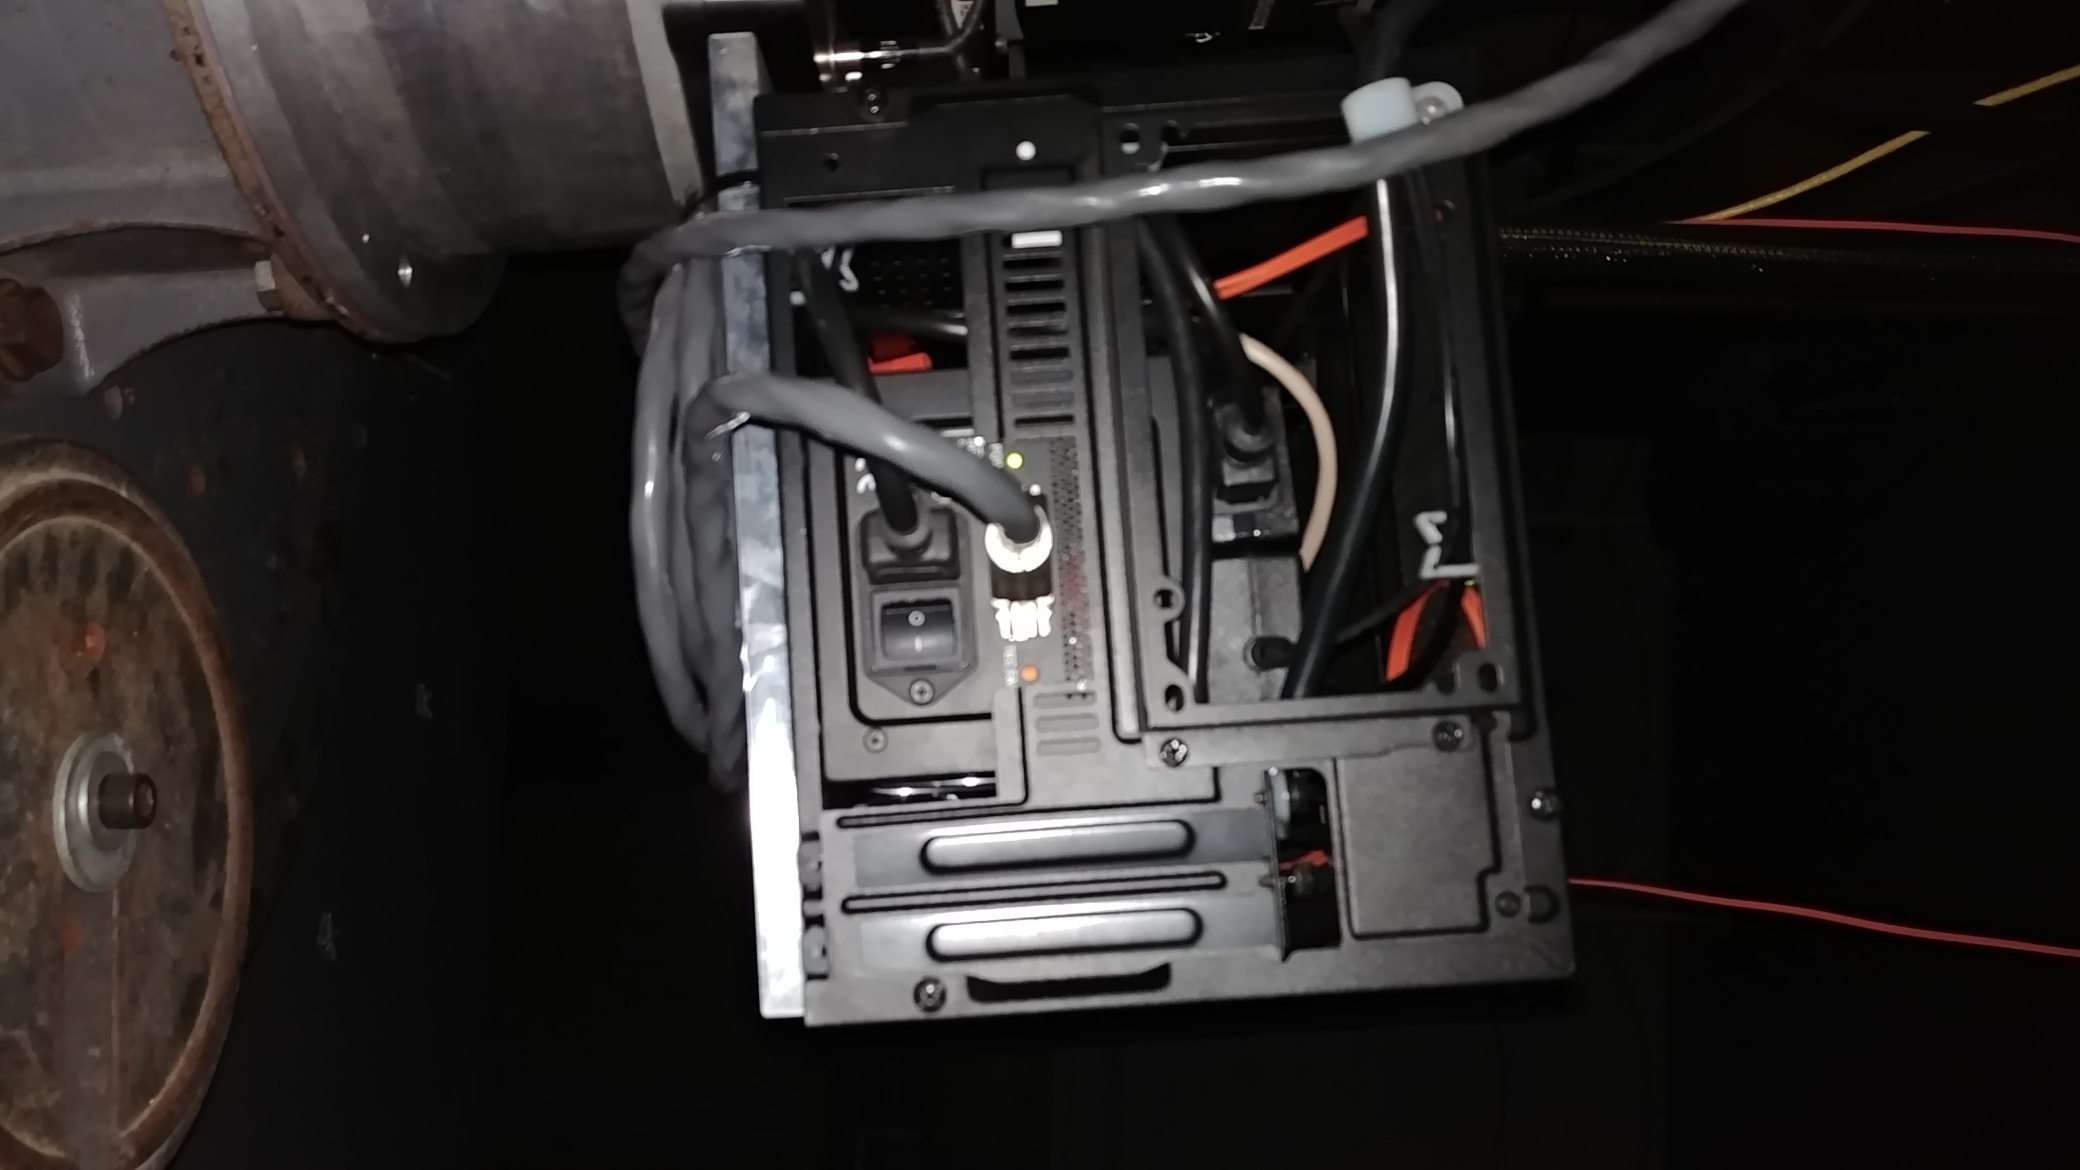
\includegraphics[width=\textwidth]{power.jpg}
  \end{minipage}
  \hfill
  \begin{minipage}[b]{0.49\textwidth}
    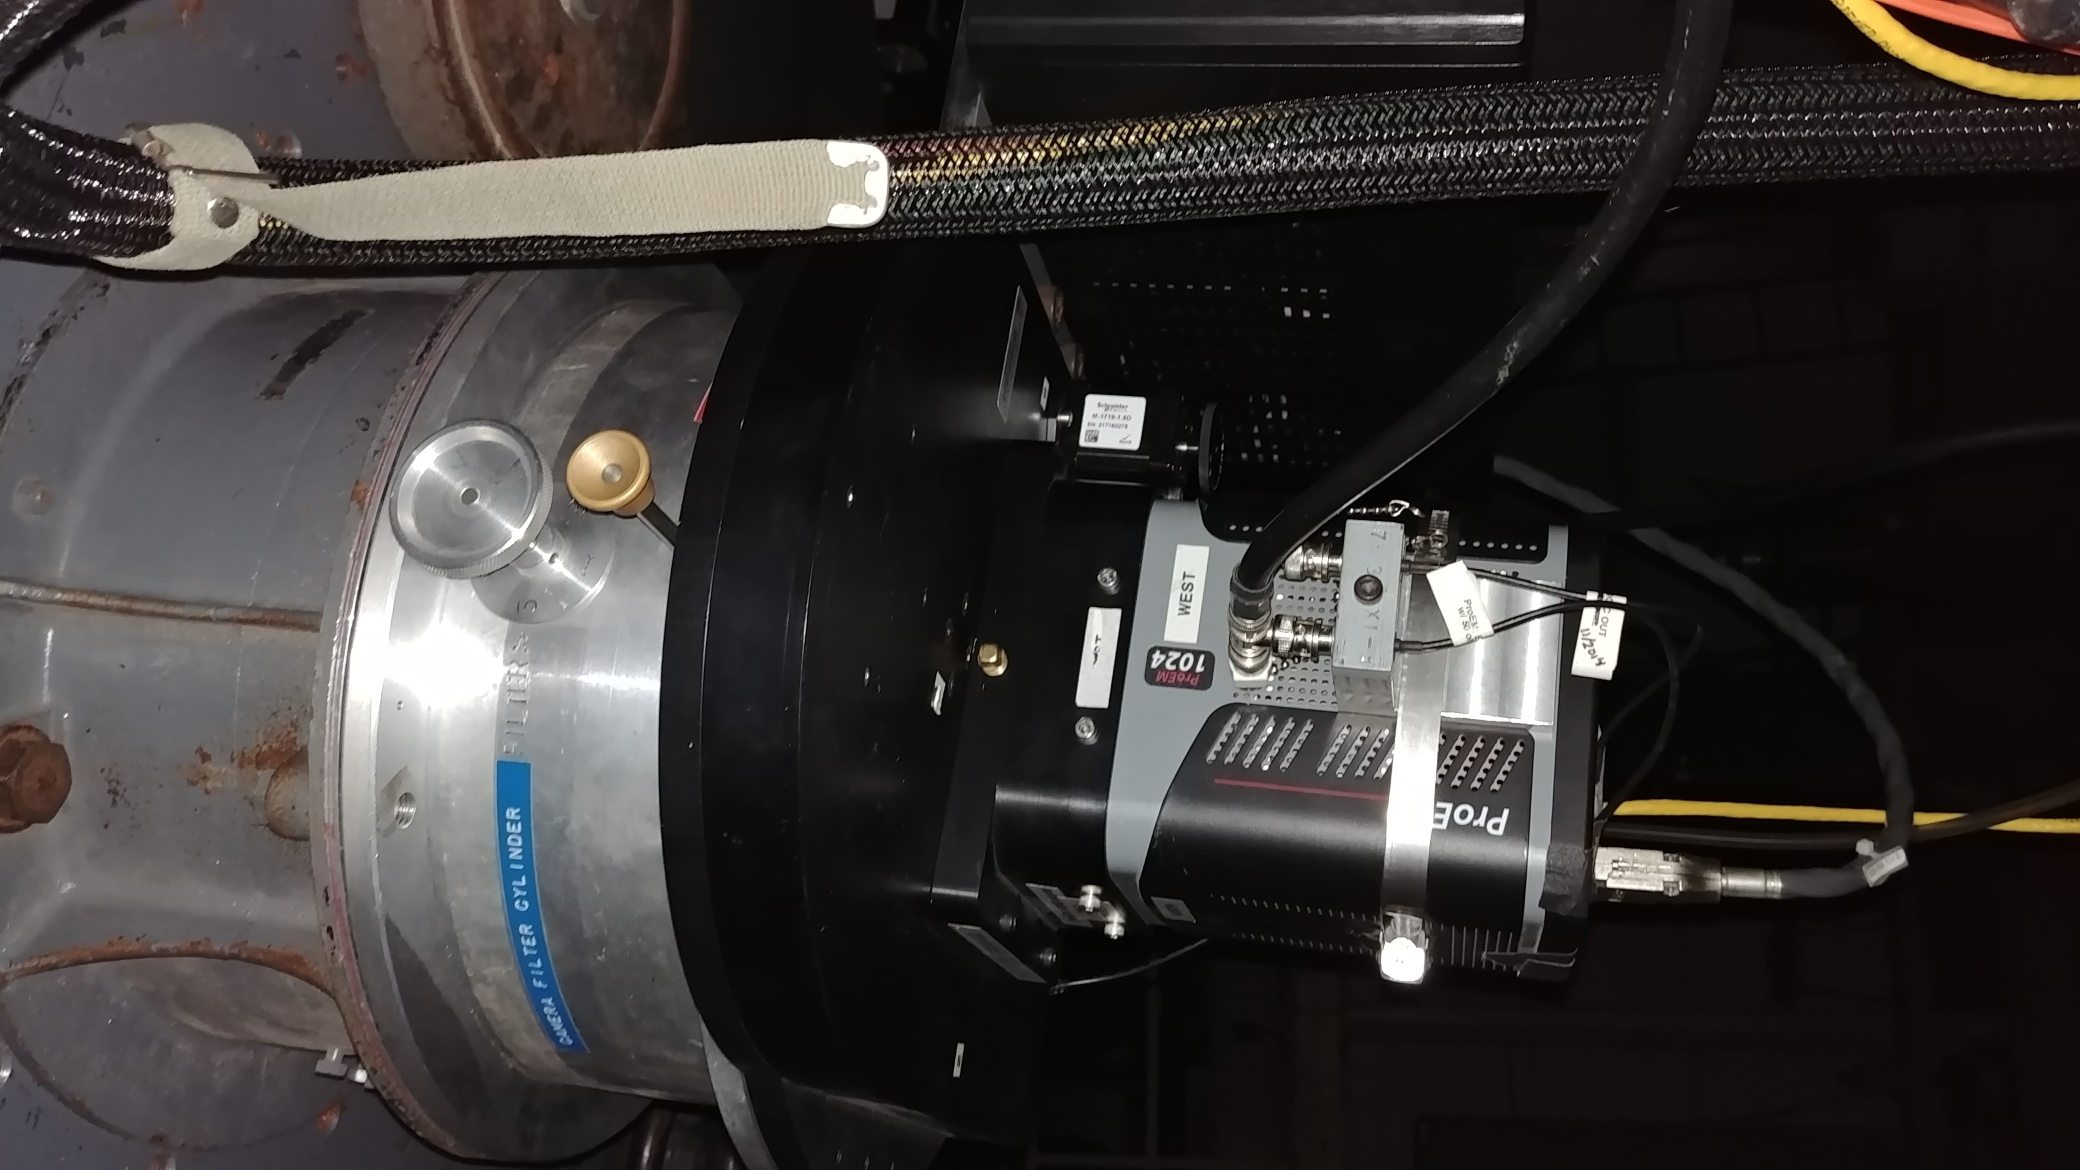
\includegraphics[width=\textwidth]{darkslide.jpg}
  \end{minipage}
  \caption{CCD connection interface and filter wheel/brass dark slide.\label{fig:ccd}}
\end{figure}

Figure~\ref{fig:ccd} shows the CCD connection interface, filter wheel, and dark slide knob. At the beginning of the night, the CCD is switched on using the power button on the connection interface. In order for light to reach the CCD, the brass dark slide knob, located above the filter wheel, must be fully retracted. Likewise, it should be inserted for taking biases, darks, and for storage at the end of the night. You can reach these if the camera is too high by raising the east platform using the hand paddle or main control console.\par
\indent The dome flat lamp is controlled by a variac box on the east side of the central telescope mount. Switch this on and slowly turn the dial to set your desired voltage (see Section~\ref{calibrations} for voltage guidelines for specific filters). When you are finished, turn the voltage down to 0V before switching the variac off.\par

\section{\textit{LightField} Software}\label{lightfield}

The control softare \textit{LightField} (Figure~\ref{fig:lf}) is run from the main computer in the warm room. An unfortunate feature of \textit{LightField} is that each image will not have its own timestamp; once data acquisition begins, there will be one absolute timestamp recorded for the beginning of the sequence, and offsets applied to calculate the rest based on your exposure time, and recorded in the footer of the .spe file. This is important to note for later, as individual image headers are not written when .spe files are converted to .fits. The program ``OLD MAID'' (discussed in Section~\ref{acquisition}) will write a .csv file with exposure timestamps for later use.\par

\begin{figure}[t]
   \centering
   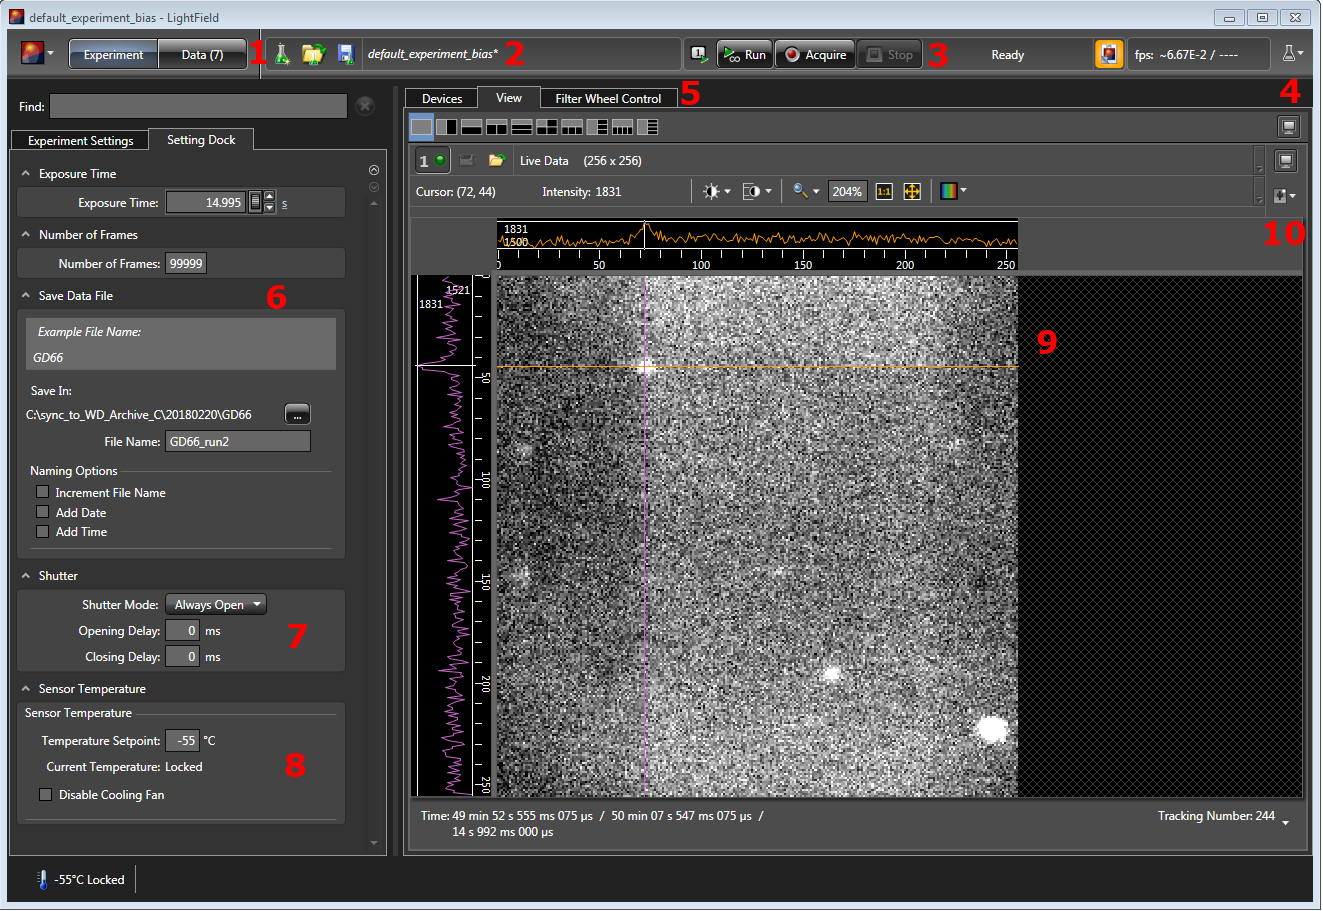
\includegraphics[width=\textwidth]{LightField_exp.PNG}
   \caption{\textit{LightField} main experiment interface.\label{fig:lf}}
\end{figure}

\noindent The following features comprise the \textit{LightField} interface:
\begin{enumerate}
   \item The ``Experiment'' tab shows current data being acquired, and the ``Data'' tab allows for review and manipulation of data.
   \item Ensure that ``default\_experiment\_bias'' is the current loaded experiment. You can do this using the ``Load Experiment'' button to the left of this field. \textbf{Never save changes to ``default\_experiment\_bias'' when closing \textit{LightField}}.
   \item The buttons ``Run,'' ``Acquire,'' and ``Stop'' control data acquisition. ``Run'' will begin taking data, but will not store it to an output file. This is useful for target acquisition, and should always be started before acquisition to allow the CCD to clean and stabilize (except for taking a filter sequence, such as for darks - see Section~\ref{calibrations}, bullet 12). ``Acquire'' will begin saving data to a .spe file. ``Stop'' will stop data acquisition.
   \item Select ``Experiment Menu,'' and then ``Show Online Statistics'' for a live readout of useful data parameters.
   \item Here you can switch between a live data readout in ``View,'' and select your observation filters in ``Filter Wheel Control'' (see Figure~\ref{fig:filters}).
   \item Here you can set your exposure time, number of frames to be taken, file location, and output file name. Note that \textbf{exposure times must be .005s less than desired} in order to compensate for the triggering mechanism. (e.g. 0.995s for 1s)
   \item Ensure that ``Shutter Mode'' is set to ``Always Open'' for taking flats and data, and ``Always Closed'' for biases, darks, and storage at end of night.
   \item Set camera temperature to -55\textdegree C at beginning of night before calibrations and wait until ``Current Temperature: Locked'' is displayed. At end of night, set temperature to approximate outside temperature (in \textdegree C) and wait until ``Current Temperature: Locked'' is displayed before shutting off CCD.
   \item Live data readout. You can position the crosshairs or draw boxes to get instant information on your data.
   \item Click ``Viewer Menu'' and check ``Always Auto-Scale'' for a consistent data display in the main window.
\end{enumerate}

\begin{figure}[b!]
   \centering
   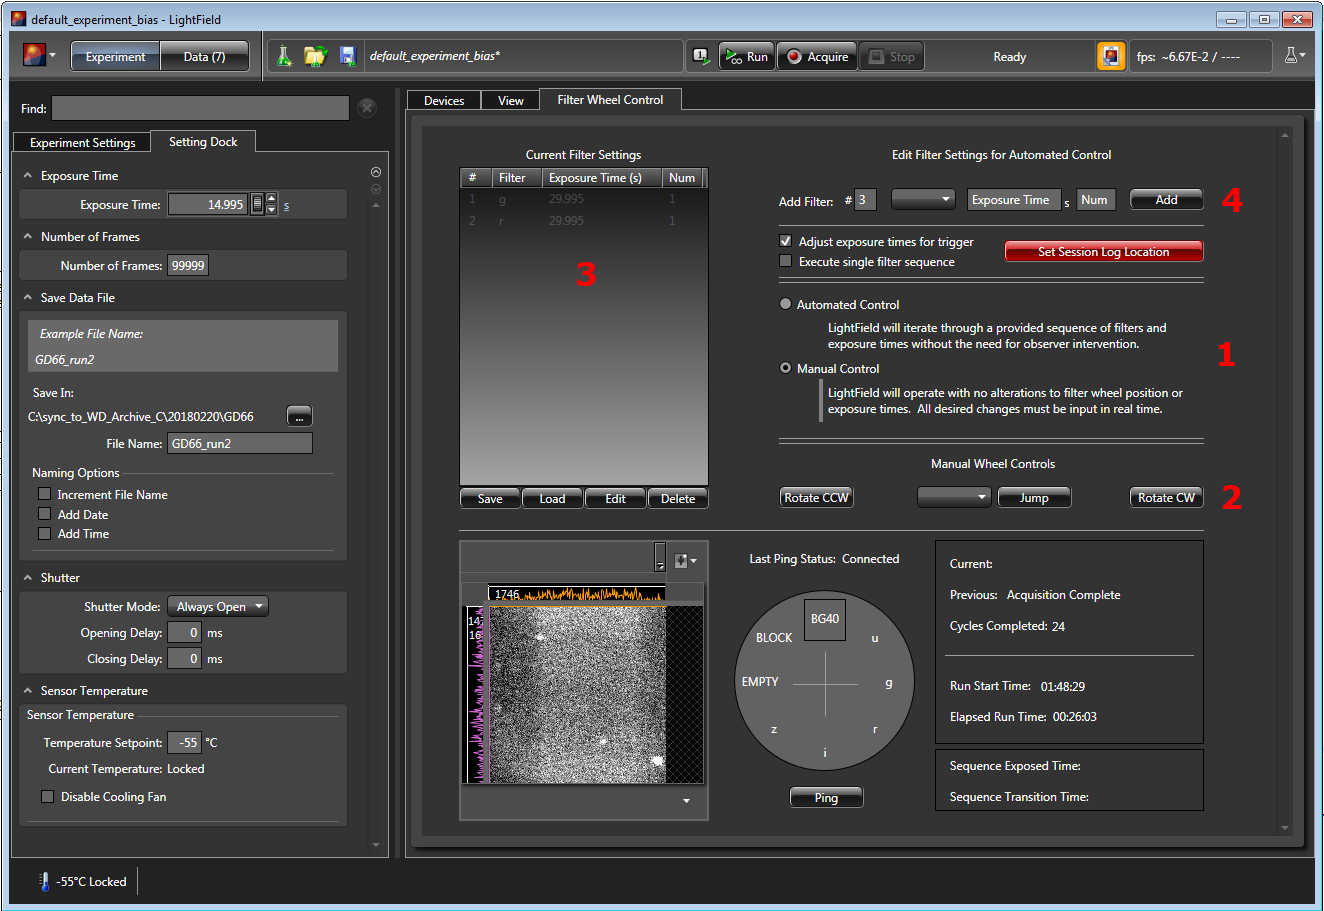
\includegraphics[width=\textwidth]{LightField_filter.PNG}
   \caption{\textit{LightField} filter wheel interface.\label{fig:filters}}
\end{figure}

\noindent Figure~\ref{fig:filters} displays the options in the filter wheel interface:
\begin{enumerate}
   \item Here you can choose between ``Manual Control'' of the filter wheel, or ``Automated Control'' where you can set a sequence of filters to execute. If one is selected, the other option will be greyed out in this interface.
   \item Here you can manually control the filter wheel. Click ``Rotate CCW'' or ``Rotate CW'' to do as such, or choose a filter from the dropdown menu at the center and click ``Jump'' to immediately jump to a filter. The telescope should always be stored with the filter set to ``BLOCK.''
   \item In automated mode, you may define a filter sequence. You may save this sequence, or load a previous one using the buttons at the bottom.
   \item Here you may define your filter sequence. Select your choice from the dropdown list, your exposure time, and number of exposures, then click ``Add.'' Below this, make sure ``Adjust exposure times for trigger'' is checked. To run your sequence once to completion, check ``Execute single filter sequence,'' or uncheck to run your cycle until manually stopped. Ensure you click ``Set Session Log Location'' and save in your current folder for later data processing. Again, \textbf{never click ``Run'' before starting a filter sequence}.
\end{enumerate}

\noindent Figure~\ref{fig:data} displays the options in the data manipulation interface:
\begin{enumerate}
   \item Here you can previously taken data (.spe) for manipulation.
   \item You can interact with your loaded data in this window as you would in the main experiment frame.
   \item At the end of the night, choose ``Export Data'' to convert your .spe data into .fits for scientific reduction.
   \item If you define an automated sequence of filters to execute, you can separate the single .spe into the component .spe files using the ``Extract Data'' button. You can select a range of frames to separate into individual files here, but they unfortunately must be consecutive - there is not yet capability to split interleaved frames within \textit{LightField}.
\end{enumerate}

\begin{figure}[t]
   \centering
   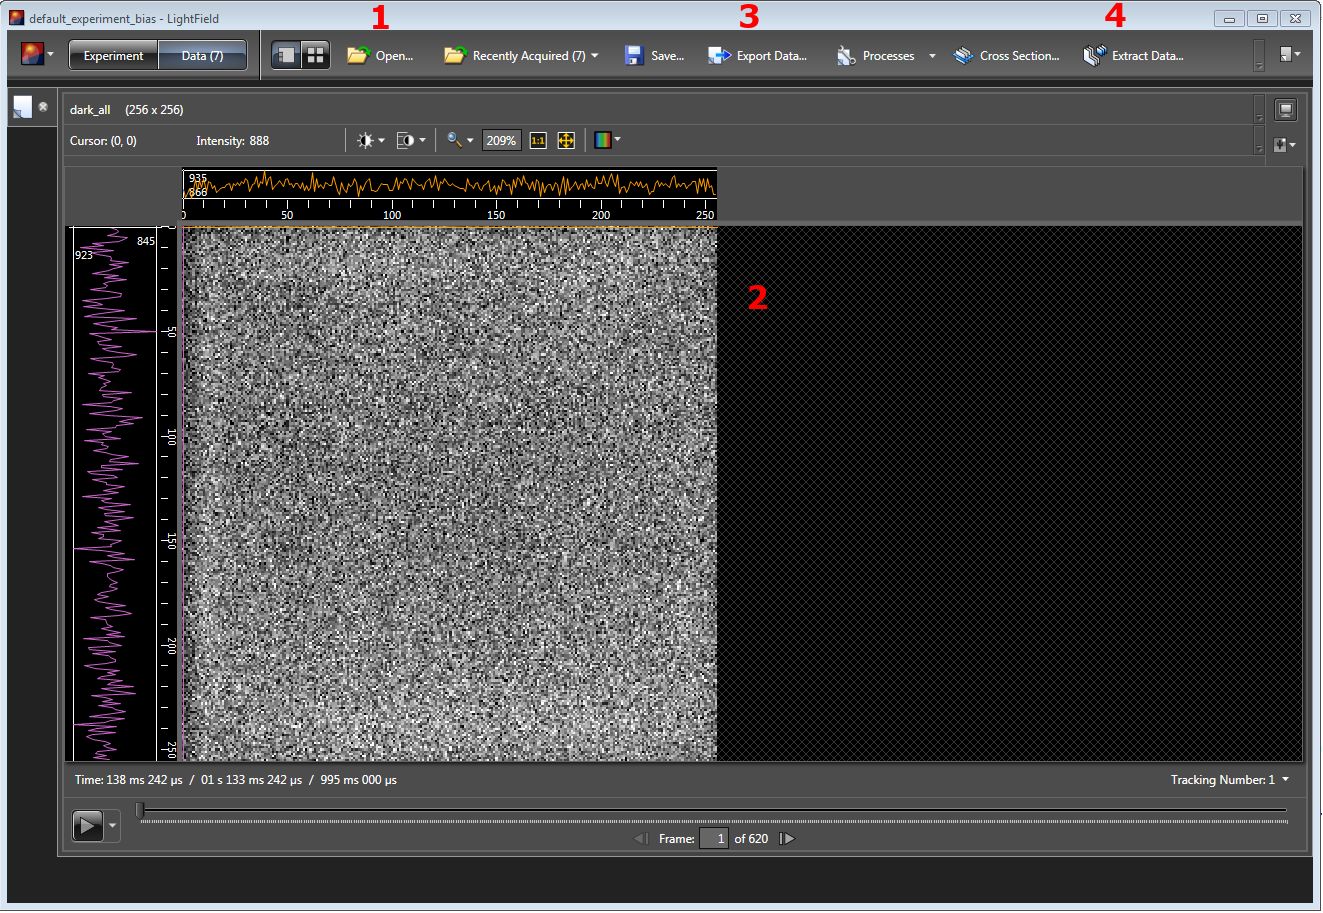
\includegraphics[width=\textwidth]{LightField_data.PNG}
   \caption{\textit{LightField} data manipulation interface.\label{fig:data}}
\end{figure}

\section{Photometric Calibrations}\label{calibrations}

\noindent\textit{\textbf{The following is your checklist for starting the telescope for calibrations at the beginning of the night:}}
\textit{(Note: In summer, it is recommended to acquire flats as close as possible to data acquisition. Therefore, it is recommended you do only biases and darks in the afternoon, and then return before sunset for flats.)}
\begin{enumerate}
   \item Switch on the telescope via the control panel.
   \item Switch on the CCD, and retract the dark slide, assuming you're doing flats first - recommended in winter, not recommended in summer. Leave the slide in and skip bullets 5-8 if you are doing your flats later.
   \item In the location C:\textbackslash\textbackslash sync\_to\_WD\_archive\_C\textbackslash, create a folder for today's date. Inside this folder, create folders called ``bias,'' ``dark,'' and ``dome\_flat."
   \item Open LightField, set camera to -55\textdegree C.
   \item Set the telescope to HA = 00:00:00, DEC = -40:00:00 (be aware this is close to the telescope pointing limit). Open the mirror cover (this takes some time) and extend the baffle.
   \item Align the ``P\&H'' logo on the dome motor with the pole on the east wall, and ensure whatever Dome Hour is shown on the computer screen is in bold (this means that the dome is set directly on a magnetic sensor). Click ``Setup'' in the bottom-center of the \textit{Guide82} window, then ``Dome,'' and then enter ``6.0'' as the custom dome hour. You will likely only need to do this the first night of your run, unless there is a power failure which resets the dome electronics.
   \item Turn on the dome lamp variac, and set to your first desired voltage for flats. You can check if you have set the variac properly using the \textit{LightField} ``Show Online Statistics'' menu - your average counts should be around 27,000. The following are approximate acceptable values and exposure times for various filters:
   \begin{itemize}
      \item BG40: 32V, 3s
      \item r: 32V, 1s
      \item g: 40V, 3s
      \item i: 24V, 1s
      \item z: 20V, 1s
   \end{itemize}
   \textit{Note: As of 5/2018 run, slightly higher voltage values were necessary to get 27,000 counts}
   \item Set your desired filter and exposure time in \textit{LightField}, and set the camera shutter to ``Always Open''. Ensure that the CCD temperature is locked at -55\textdegree C, choose the path to your ``dome\_flat'' folder, enter a filename for your flats (e.g. ``dome\_flat\_BG40\_3s"), and click ``Run'' to begin previewing your flats. Check that you are receiving 27,000 average counts in the ``Show Online Statistics'' window. If you are satisfied, you may  begin acquiring. 61 flats are recommended per setup.
   \item Once you have finished taking flats for all your setups, set the camera shutter to ``Always Closed,'' set the CCD filter to ``BLOCK,'' re-insert the dark slide, and point the telescope to RA = 00:00:00, DEC = -20:00:00. Retract the baffle and close the mirror cover.
   \item In \textit{LightField}, set exposure time to 0, choose the path to your ``bias'' folder, change your filename to ``bias,'' and click ``Run'' to begin taking biases. Ensure average counts are around 900, and then acquire 61 bias images.
   \item Once biases are completed, choose the ``dark'' path and change your filename to ``dark\_all.'' Now it is recommended to define a sequence of darks to take while you return to the lodge for dinner. The typical sequence can be loaded by locating the file ``Filter\_Settings.dat'' in any previous night's dark directory. Copy this file to your current dark directory each night for easy location in the future.\\
   If you need to define the series yourself, the recommended sequence is: 1s x10, 1s x61, 2s x61, 3s x61, 5s x61, 8s x61, 10s x61, 15s x31, 20s x31, 30s x31, 60s x31.
   \item Check ``Execute single filter sequence'' and ``Adjust exposure times for trigger'' if you entered whole number exposure times. Click ``Set Session Log Location'' and save the resulting file to the ``dark'' folder. Then click ``Acquire'' directly (NOT RUN), as this file will begin logging dark information (the first 10 files in the recommended sequence are throwaway, and will take the place of the Run function). Once you are sure your darks are acquiring properly, you may return to the lodge for dinner. The recommended dark sequence should take about an hour and a half to complete.
   \item Once you return to the dome and your darks are completed, use the ``Extract Data'' function to split ``dark\_all.spe'' into the component darks. Choose the range of frames to save as each set of darks based on exposure time (e.g. after ignoring the first 10 throwaway images, ``dark\_1s'' will be frames 11-71, ``dark\_2s'' will be 62-132, etc.). If you have not taken flats, do them now.
\end{enumerate}


\section{Data Acquisition}\label{acquisition}
\textit{Open the doors in the dome to assist in temperature normalization when you return at sunset.}\par
Create a folder for each new object in your current day's directory, and instruct \textit{LightField} to save your object data to that folder. For each target, it is recommended that you update a running text file log for the night, and a more detailed one for each target (see previous nights for a template of each which you can alter for your current nights' data). Current weather information including temperature, relative humidity, and wind speed is read out every 5 minutes on the monitor on top of the set of computers against the window. Also, note the weather alert panel on the wall to the right of this monitor - \textbf{if this alert is ever triggered, close the dome immediately} and report in the night report.\par
\indent You will need to manually slew the telescope onto your targets if they are a significant distance away from your current position. Once you are close, final pointing is completed using the pointing/guiding/focusing program (see Figure~\ref{fig:point}) on the computer screen in the dome or on the computer opposite the one running \textit{LightField} in the warm room. For each of these computers, you must hold the shift key as a safety switch to complete any movement as you would the pedal on the main telescope console or the trigger button on the hand paddles.\par

\begin{figure}[!t]
   \centering
   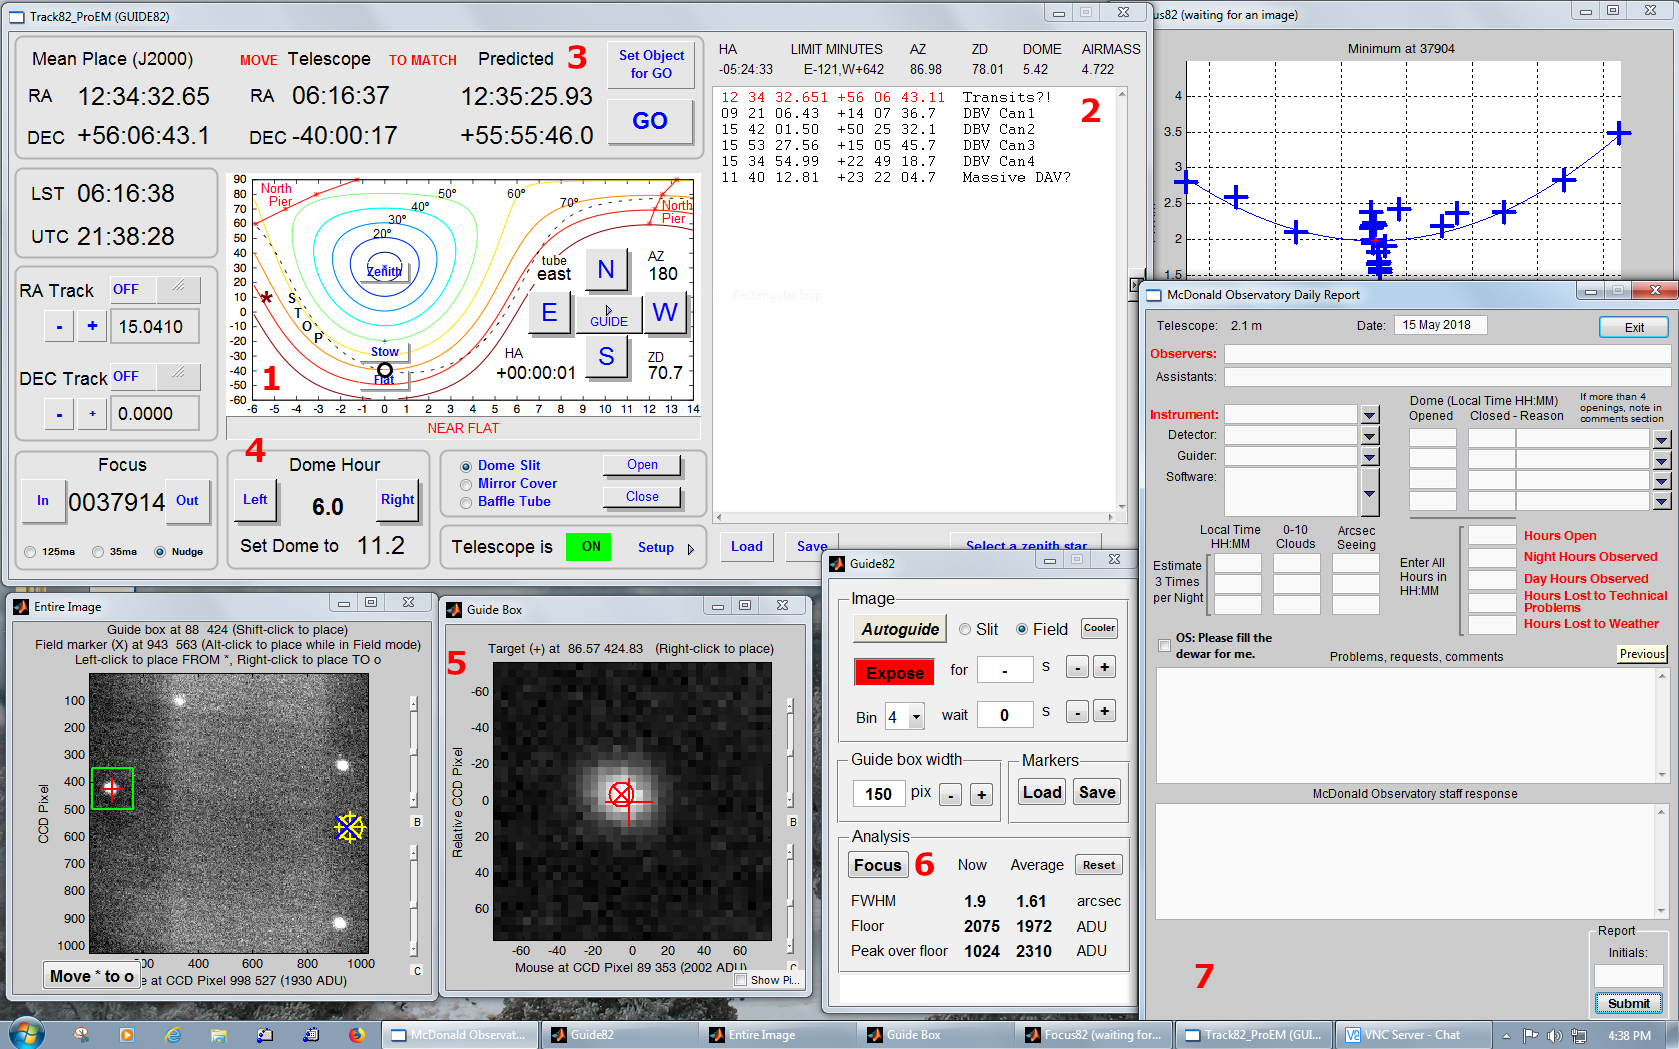
\includegraphics[width=\textwidth]{pointing.png}
   \caption{Telescope pointing, guiding, and focusing interface.\label{fig:point}}
\end{figure}

\noindent The following are the features of the telescope pointing, guiding, and focusing interface:
\begin{enumerate}
   \item This chart displays the current telescope position on the sky (circle), the location of your specified object (star), and the limits of the telescope (dashed line). Also marked are the stow position 00:00:00 -20:00:00, flat position 00:00:00 -40:00:00, and zenith.
   \item Here you may input object coordinates in RA and DEC. Set the cursor within your typed coordinates and they will turn red. Then you can click "Set Object for Go" to send these coordinates to the computer in the dome.
   \item If slewing is necessary to reach your target quickly, in the dome, slew as close as possible to the ``Predicted'' position. Once you are close, turn on RA tracking (left of this program), hold the shift key and click ``Go'' to finish accurate pointing (hold shift until the program announces ``On Target''). If your object is already close to the object position, you may use ``Go'' from the warm room to switch targets. You may make desired adjustments to your field of view using the paddle by the \textit{LightField} computer.
   \item Here you may rotate the dome (while holding the shift key). This will also report to which hour you should rotate the dome to position your target in the slit. It is recommended that you keep your current dome hour within 0.6 of the predicted value for your target to avoid tracking into the dome. If the number is bolded, the dome is currently sitting directly on a magnetic sensor. The ``Setup'' button next to the telescope status indicator to the right allows you to set the dome hour yourself (see Section~\ref{calibrations}, bullet 6)
   \item These windows will help you to establish guiding once you send acquiring data from the \textit{LightField} computer (see paragraph following this list). Use shift-click to place the green box on the brightest object in your field, and this zoomed area will appear on the window to the right of your image preview. In the zoomed window, right-click to place the red crosshairs on your guiding target. The program will then attempt to place your guiding target on the crosshairs in each successive image. Once you are happy with your placement, click ``Autoguide'' in the window to the right of the zoomed view to complete. When you switch objects, ensure that you turn off ``Autoguide'' so that you can place a new box and crosshair for your new object.
   \item Clicking the ``focus'' button in this window will bring up a plot to help you determine an optimal focus value for the night (top-right of Figure~\ref{fig:point} - close the last night's if it is still open). Before starting this, shift-click to move the focus ``In'' and set your image well out-of-focus. Double-clicking will move the focus value faster, as will selecting larger increments from the options under the current value. Then, click the ``focus'' button, and allow a new image to be transferred from the \textit{LightField} computer. Once the image is received here, it will place a mark on the focus plot. Move your focus ``Out'' slightly, and wait for another image to come in and a mark to be placed. Repeat this until you have turned past a focus minimum on the plot, then click the plot area to fit a parabola to your data points and receive an optimal focus value. You may then set the focus to this optimal value and continue data acquisition for the rest of the night. The optimal value should also be recorded in the night log. This box will also report an approximate seeing value for each new image, and the seeing should be recorded three times per night in the night report on this computer. Click ``reset'' for each new object to get seeing values for that object alone.
   \item This is the night report for the observatory staff. Record your name, the instrument you are using (``ARGOS,'' ``ProEM,'' ``LightField,'' ``Guide82''), any times that you open or close the dome and for what reason (weather, wind, clouds, etc.), the seeing value at three points throughout the night, your time breakdown for the night, and complete it by signing your initials, but \textbf{do not submit}. The observatory staff will confirm and submit this report the next day.
\end{enumerate}

There are two additional programs on the \textit{LightField} computer which are used for data acquisition, and they are immediately underneath \textit{LightField} on the desktop. The first one, called ``OLD MAID,'' is used for live light curve production and Fourier transform fitting, and the second is used to send data to the guiding computer. Run this second program first, and choose your currently-acquiring .spe file to send over. Once you have established guiding, return and run OLD MAID. Here, you may load in your current .spe file, and apply darks, flats, and darks for flats (use the appropriate split dark .spe files for your image and flat exposure times). Then click your target in the image preview window, followed by comparison stars in order of priority (i.e. click brighter comparison stars first). Once your target and comparison stars are selected, click File\textgreater Run Photometry to begin live light curve production. Once you stop acquisition in \textit{LightField}, OLD MAID will save a screenshot of the final light curve and FT, as well as a list of image timestamps to your current object folder. \textbf{This timestamp file is necessary to record accurate image headers, so ensure that it is saved.} Running OLD MAID again on your .spe will re-generate it if there is a failure.

\section{End of Night}\label{end}
\textit{\textbf{The following is your checklist for ending your night and safe telescope storage:}}
\begin{enumerate}
   \item Turn off Autoguiding and RA Tracking on the guiding computer.
   \item Park the telescope as close as possible to HA = 00:00:00, DEC = -20:00:00. Retract the baffle and close the mirror cover.
   \item Close the dome slit, and set the upper windscreen directly overhead to shield the telescope from possible rain. Return the dome to hour 6.0 (bolded).
   \item Warm the CCD to ambient dome temperature (estimate based on the weather monitor screen above the guiding computer, and note that \textit{LightField} accepts values in \textdegree C). Wait for temperature to be locked, set shutter to ``Always Closed,'' Set filter wheel to ``BLOCK,'' switch off the CCD, and insert the dark slide.
   \item Power off the telescope via the main control panel. (This will make the Pacman death noise)
   \item All logs should be completed with accurate timestamps from the OLD MAID .csv files.
   \item Convert all .spe files into .fits files for data reduction using the ``Export Data'' option in \textit{LightField} (see Fig.~\ref{fig:data}, bullet 3). Add the current day's directory to the window to the left, and check ``Include all sub-directories'' before finishing. Transfer your night's folder from C: to D:. You can also transfer data to a remote destination using the \textit{WinSCP} program on the desktop.
   \item Shut down OLD MAID, the data transfer program, and \textit{LightField}.
   \item Complete the night report, but do not submit.
\end{enumerate}

\hfill \\

\section{Miscellaneous Errors and How to Fix Them}
\textit{List to be continually updated! Please report any new errors you face here.}
\begin{itemize}
   \item If \textit{LightField} crashes on the splash screen, this is typically associated with a loss of connection to the D: drive. Reboot the computer, and login as ``admin''; the drive should hopefully reconnect on boot. The password is on the back of the computer tower (\textit{Note: The lowercase o's are actually zeros!}). The password for the ccd account on the dome slit computer is also listed here, should that be logged out.\\
   \textit{As of 2018-05-21, John Kuehne has removed D: entirely. UNC observers need not use D:, as we can scp our data to Chapel Hill, so it is recommended you just keep everything on C: and transfer to AFS at the end of the night.}
   \item If the dome will not rotate, try to move it in the opposite direction, and then back in the desired direction with some speed to overcome whatever hiccup is in the track.
   \item Should there be a power outage or a fuse break, enter the small room on the north wall and go to the breaker cabinet on the back-left wall. Near the bottom of this cabinet is a large green button that says RESET. If this does not fix the problem, call for help!
   \item If connection is lost to the filter wheel, try clicking ``Ping'' in the filter wheel menu of \textit{LightField} to attempt reconnection. If this fails, check all connections to the filter wheel in the dome. This may require a full reboot of the filter wheel computer, which requires assistance from Zach Vanderbosch, John Kuehne, or Coyne Gibson.
\end{itemize}

\end{document}
